%%% Sekce – Závěr
%%%%% Wording: ✅
%%%%% Styling: ✅
%%%%% References: ✅
%%% --------------------------------------------------------------
\section{Závěr}
\label{sec:implementace-zaver}
Tato kapitola nabídla komplexní přehled rozhodovacího procesu a strategického uvažování, které se podíleli na vývoji aplikace pro webové řešení prodeje vstupenek s rezervací míst pomocí moderních webových technologií.
Objasňuje složitou cestu vytváření sofistikované frontendové aplikace od jejího počátku s pečlivými vysvětleními poskytnutými pro každou následující fázi.

Počáteční fáze zahrnovala rozhodnutí o technologickém stacku, který upřednostňuje sílu Reactu a TypeScriptu pro vytvoření škálovatelné a udržovatelné aplikace.
Architektura a struktura projektu byly metodicky uspořádány podle moderních nejlepších postupů s ohledem na potenciální růst projektu.

Kapitola primárně analyzovala čtyři hlavní funkce celého řešení, konkrétně interaktivní mapu sedadel, správu košíku, rezervační systém a proces dokočení objednávky, aby bylo možné důkladně porozumět strategiím použitým při jejich implementaci.
Tyto funkce se s důrazem na uživatelský zážitek snaží zpříjemnit a zjednodušit proces rezervace vstupenek.

Interaktivní mapa sedadel tvoří jádro aplikace, ilustruje dynamické použití manipulace s \ac{svg} strukturou a poskytuje uživatelům intuitivní způsob výběru sedadel.
Následující sekce podrobně popisují správu nákupního košíku, rezervačního systému a procesu dokočení objednávky, které jsou všechny úzce propojeny s mapou sedadel.

Konečným výsledkem je funkční prototyp, který demonstruje všechny hlavní funkce, které byly v této kapitole analyzovány a je k dispozici na cloudové platformě Vercel.

Je důležité poznamenat, že tato aplikace funguje pouze jako prototyp, který se hladce integruje se simulovaným \ac{api}, a různé další praktické aspekty, jako je zabezpečení, optimalizace výkonu, důkladná správa chyb či internalizace\footnote{Internalizace je proces přizpůsobení aplikace pro použití v různých jazycích a regionech.}, mohou vyžadovat další zvážení při vývoji aplikace připravené k produkci.

Souhrnně tato kapitola ilustruje, jak moderní technologie jako React a TypeScript, spolu s promyšleným plánováním, strategickým uvažováním a metodickým přístupem, mohou být úspěšně použity k vytvoření sofistikované frontendové aplikace.

Finální podoba nákupního procesu v rámci nasazené aplikace je zobrazena na obrázích~\ref{fig:final-flow}

\begin{figure}[h]
    \centering
    \hfill
    \begin{subfigure}{0.48\textwidth}
        
\includegraphics[width=\textwidth]{\FIGDIR/final-flow-venue-loading}
        \caption{1 - Načítání sálu}
        \label{fig:final-flow-venue-loading}
    \end{subfigure}
    \hfill
    \begin{subfigure}{0.48\textwidth}
        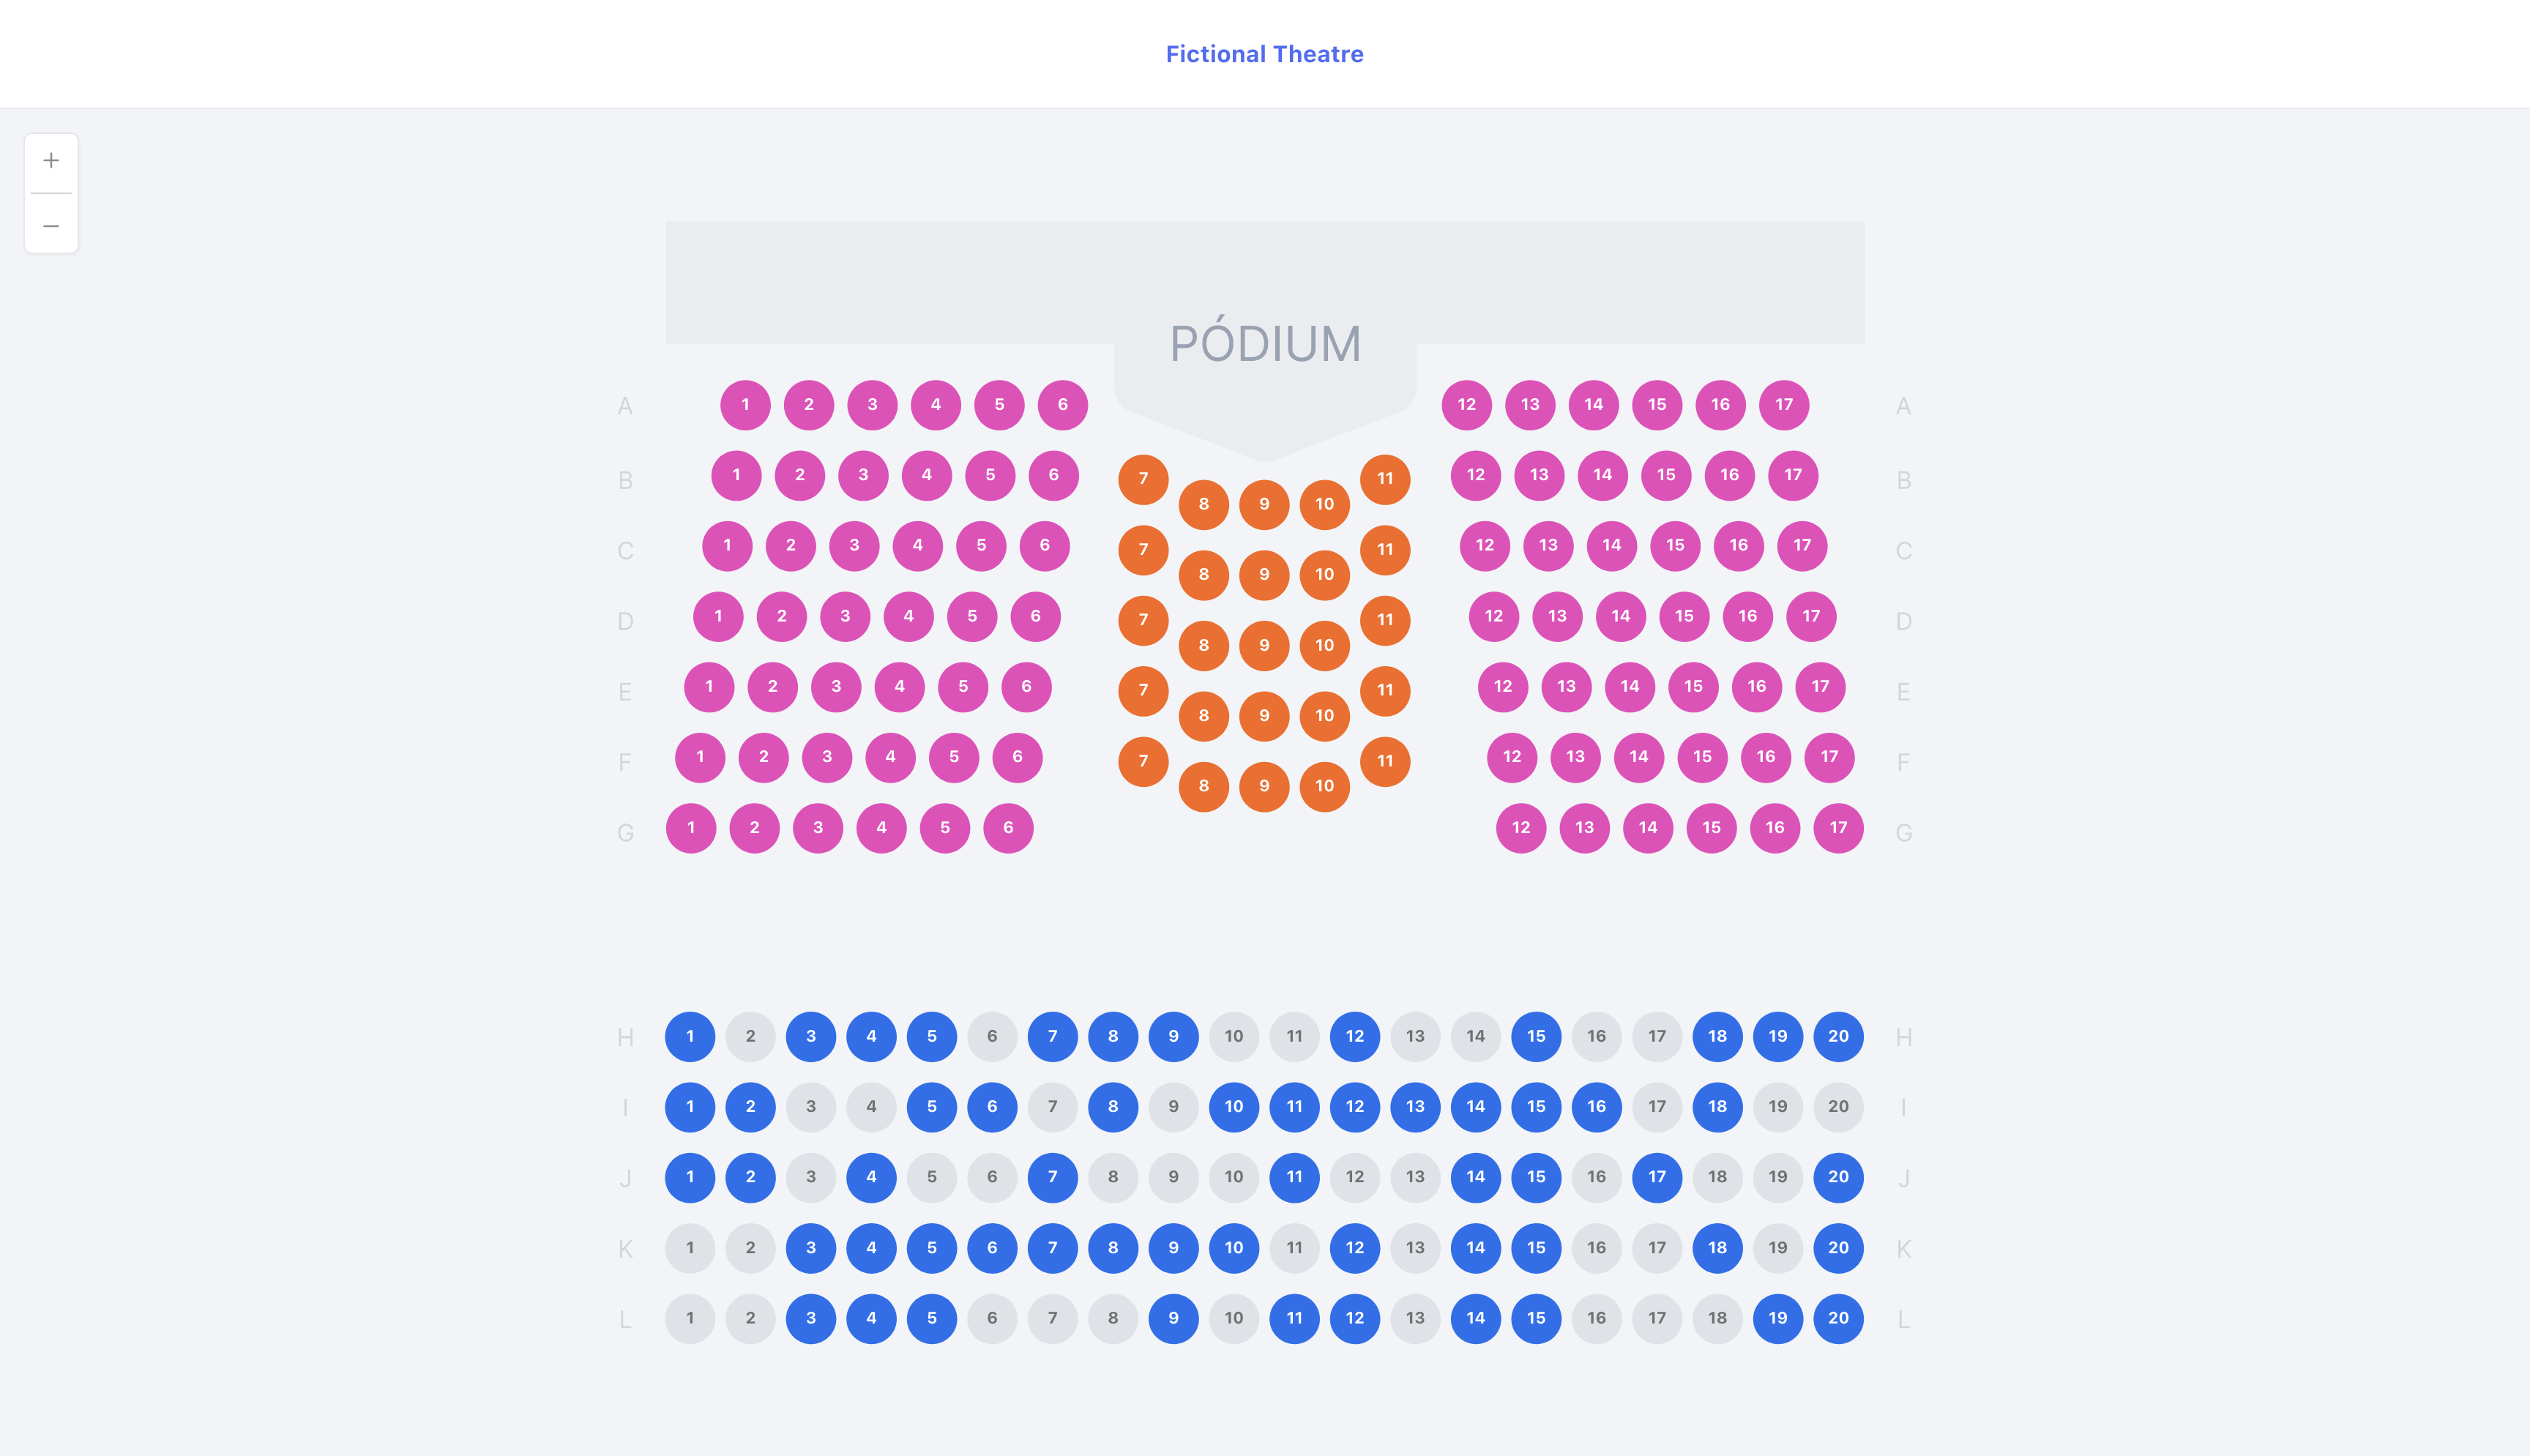
\includegraphics[width=\textwidth]{\FIGDIR/final-flow-seating-map}
        \caption{2 - Interaktivní mapa sedadel}
        \label{fig:final-flow-seating-map}
    \end{subfigure}
    \hfill
    \begin{subfigure}{0.48\textwidth}
        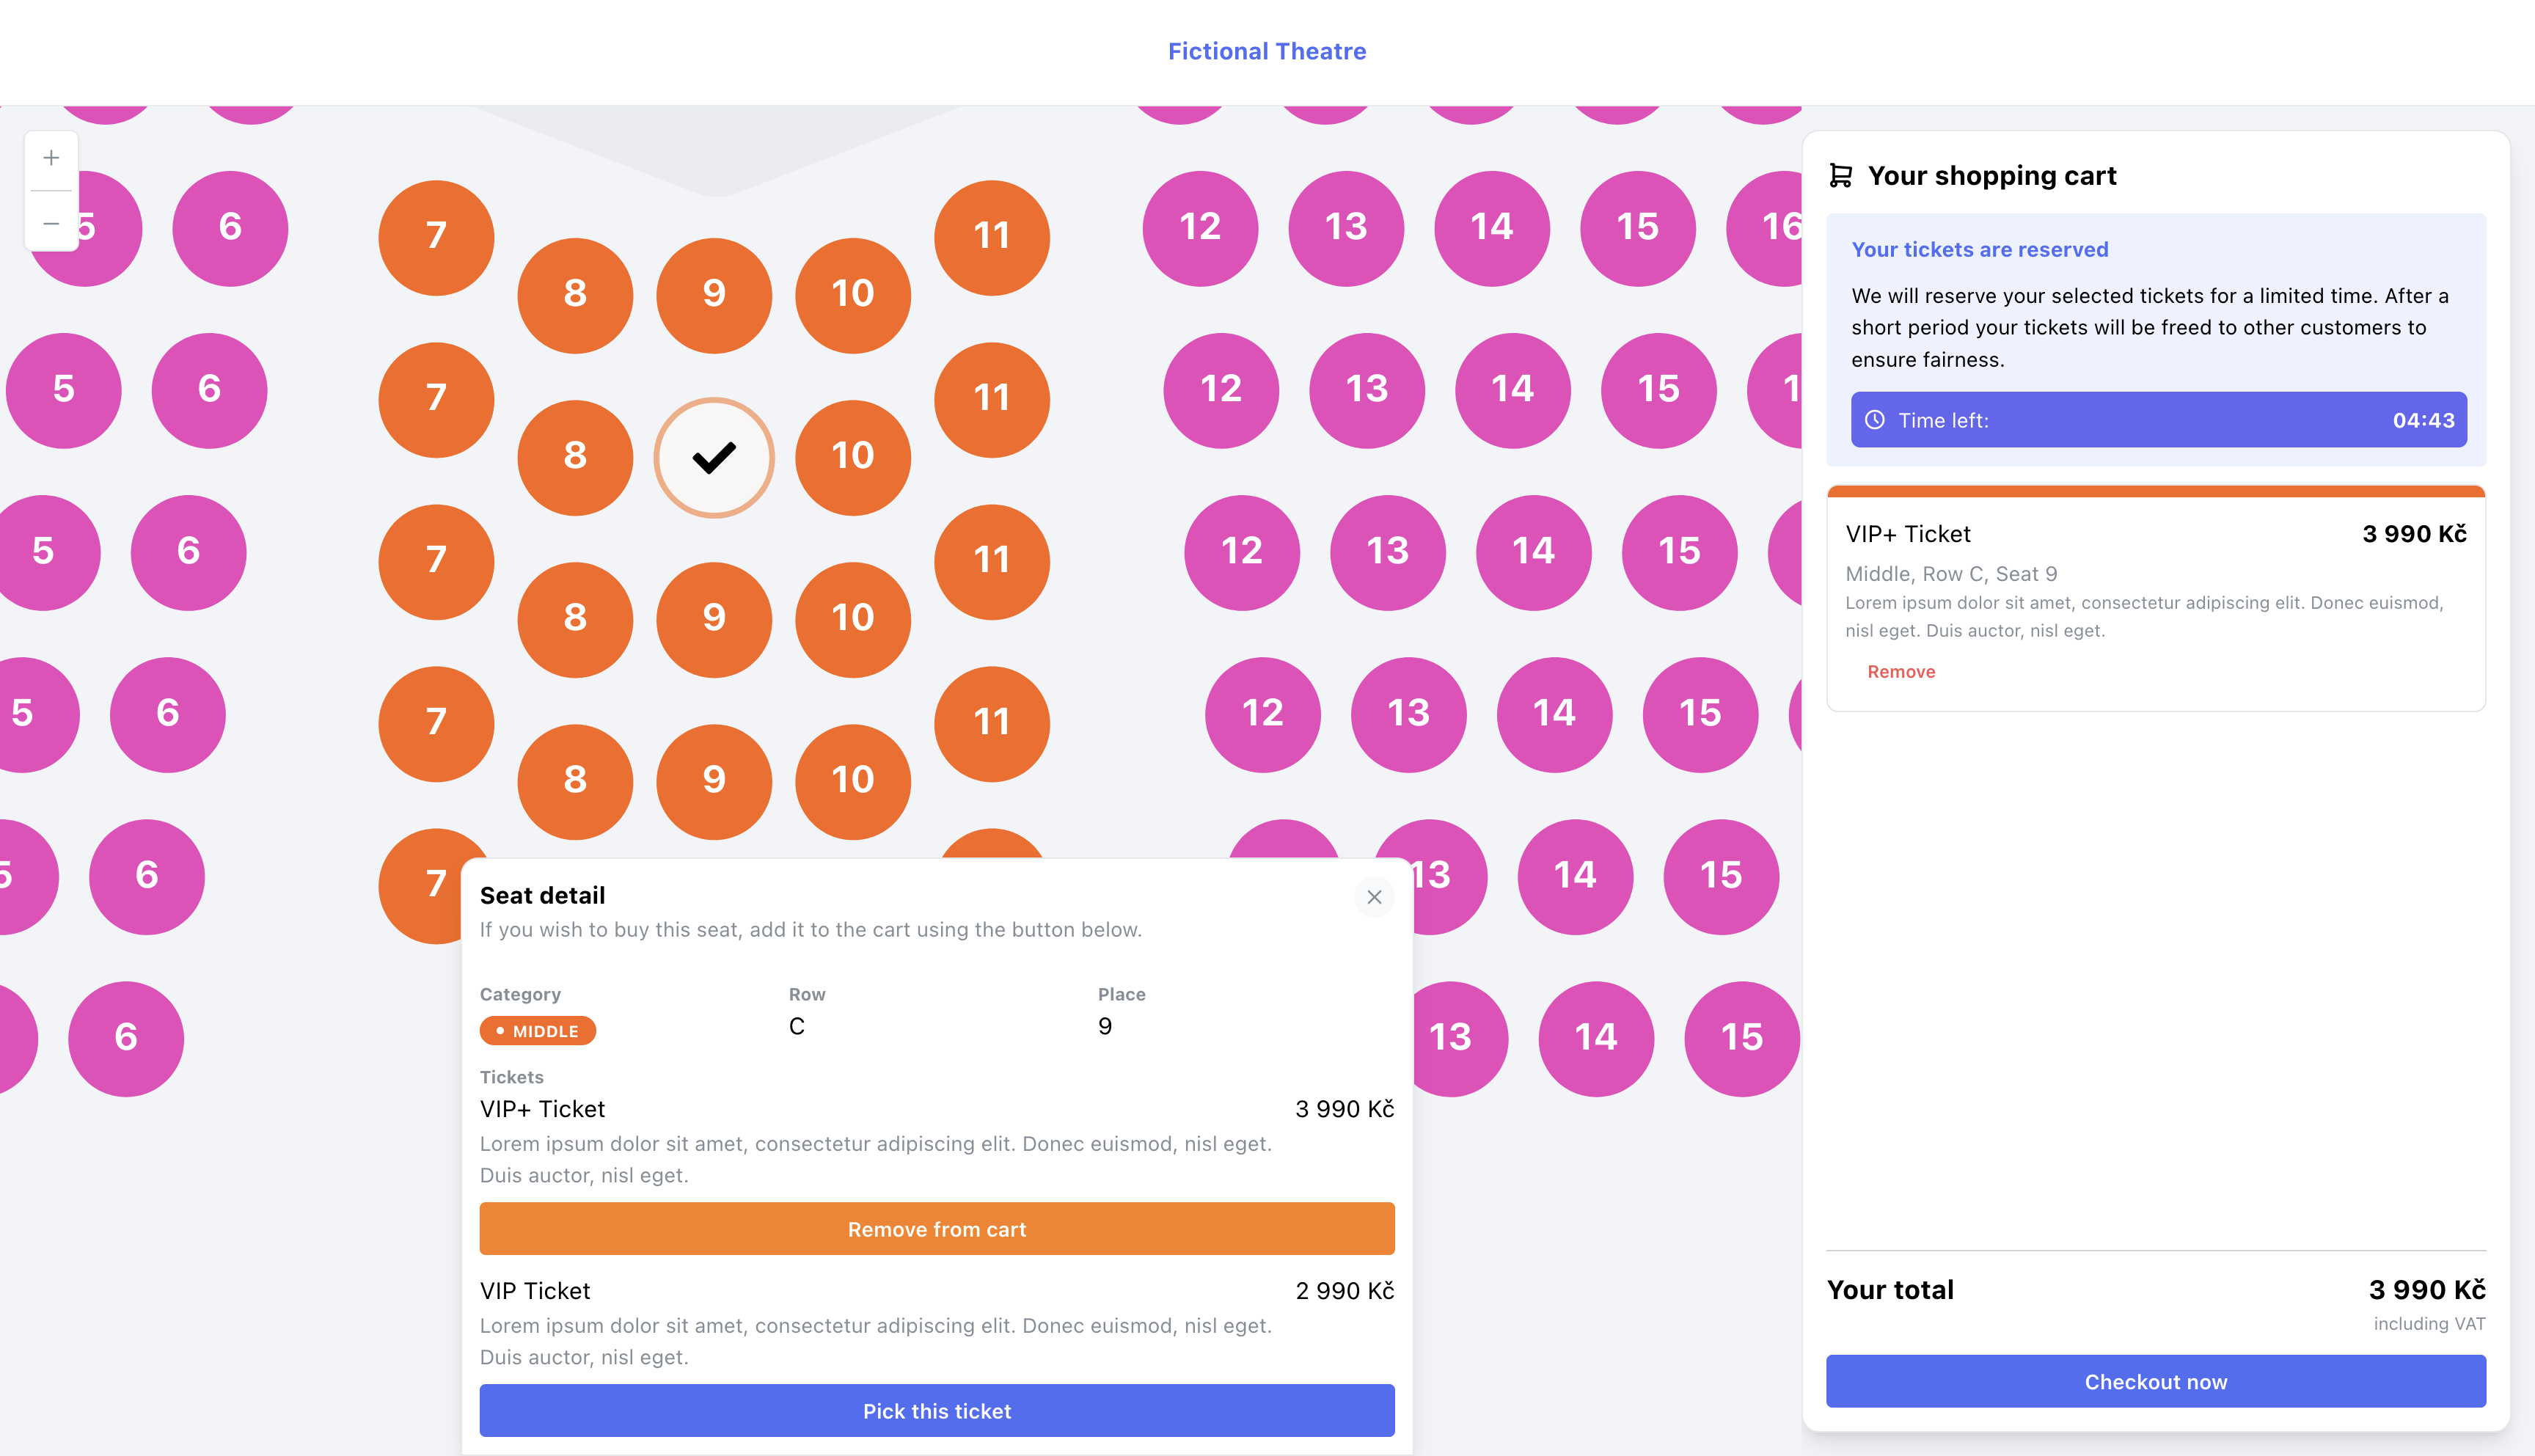
\includegraphics[width=\textwidth]{\FIGDIR/final-flow-seat-selection}
        \caption{3 - Výběr sedadel}
        \label{fig:final-flow-seat-selection}
    \end{subfigure}
    \hfill
    \begin{subfigure}{0.48\textwidth}
        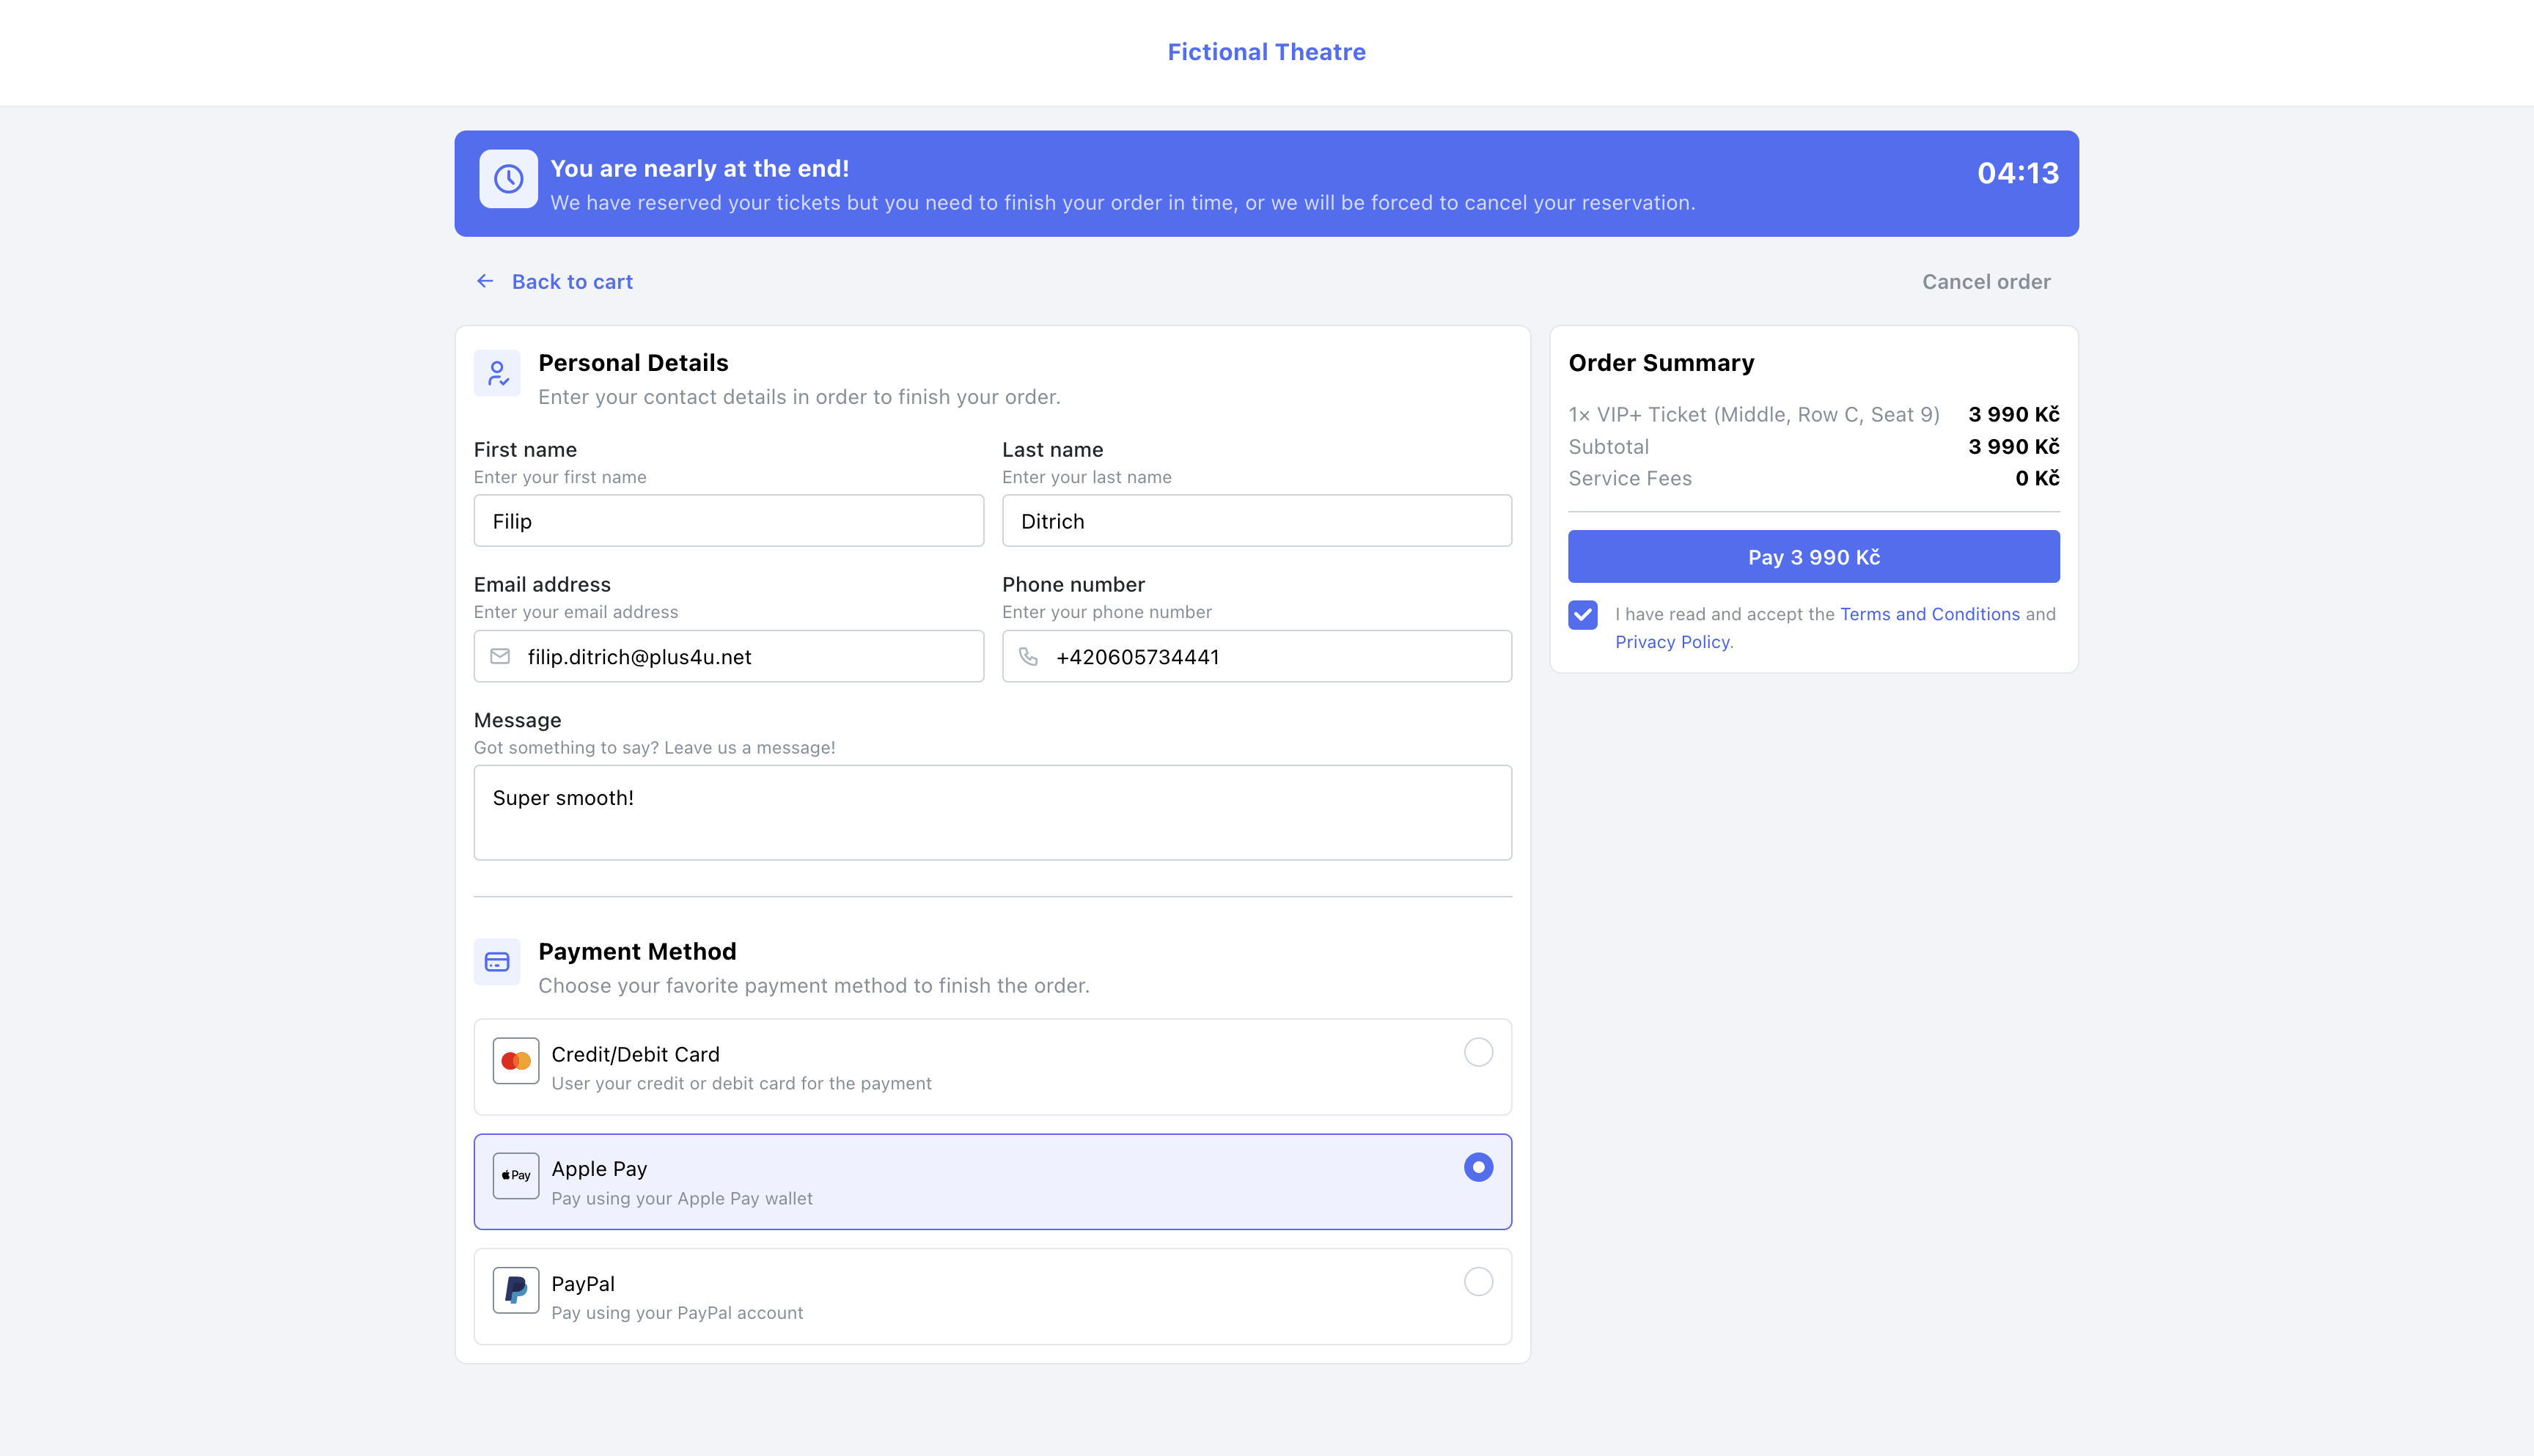
\includegraphics[width=\textwidth]{\FIGDIR/final-flow-checkout}
        \caption{4 - Dokončení objednávky}
        \label{fig:final-flow-checkout}
    \end{subfigure}
    \hfill
    \begin{subfigure}{0.48\textwidth}
        
\includegraphics[width=\textwidth]{\FIGDIR/final-flow-order-processing}
        \caption{5 - Zpracování objednávky}
        \label{fig:final-flow-order-processing}
    \end{subfigure}
    \hfill
    \begin{subfigure}{0.48\textwidth}
        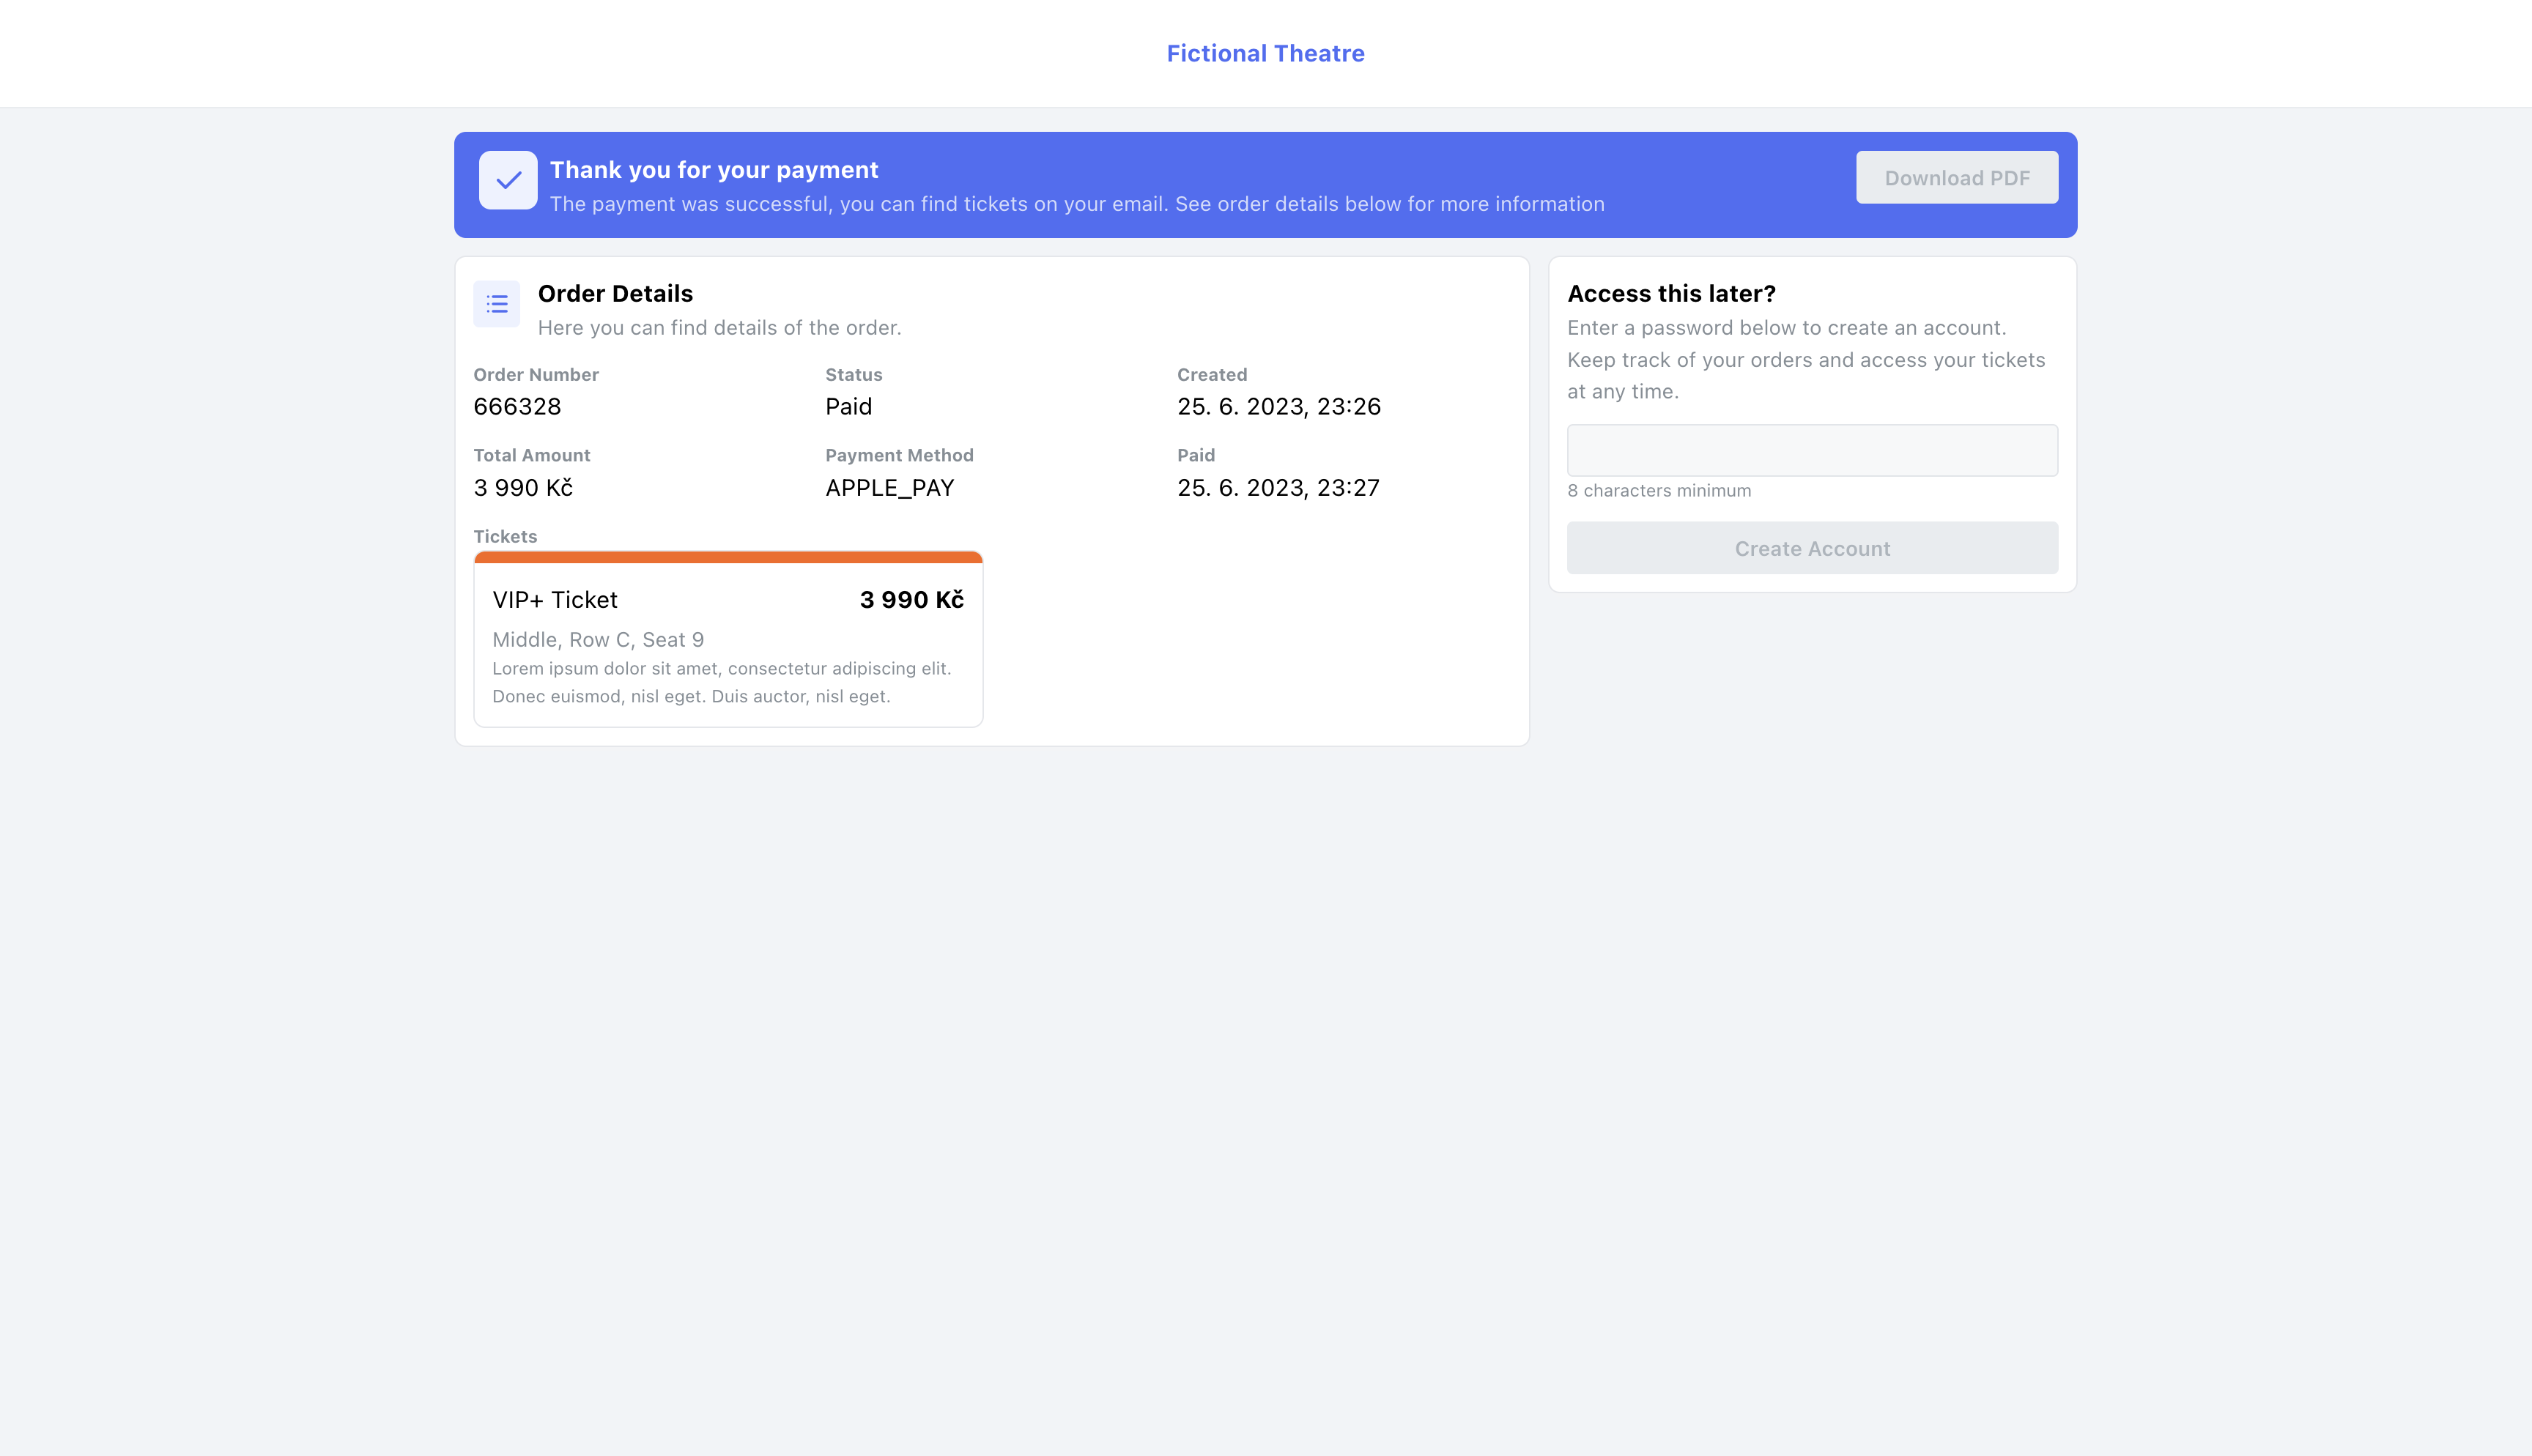
\includegraphics[width=\textwidth]{\FIGDIR/final-flow-order-confirmation}
        \caption{6 - Potvrzení objednávky}
        \label{fig:final-flow-order-confirmation}
    \end{subfigure}
    \caption{Kompletní nákupní proces}
    \label{fig:final-flow}
\end{figure}

Následující kapitola pojednávajá o zajímavých problémech, které se dále vyskytly během vývoje tohoto projektu, o použitých strategiích k jejich překonání a o získaných zkušenostech.
Reflexe této cesty poskytuje cenné poznatky a vodítko pro budoucí projekty podobného charakteru.
